\documentclass[a4paper]{article}
\usepackage[a4paper,margin=0mm]{geometry}
\usepackage{fontspec}
\usepackage{unicode-math}
\usepackage{tikz}
\usetikzlibrary{calc}
\usepackage[table]{xcolor}
\usepackage[absolute]{textpos}
\usepackage{enumitem}
\usepackage{array}
\usepackage{multirow}

\setmainfont{Libertinus Serif}
\setsansfont{Libertinus Sans}
\setmathfont{Libertinus Math}

\definecolor{accent}{HTML}{0F6A52}
\definecolor{badge}{HTML}{A9CFC2}
\definecolor{ink}{HTML}{2A2E30}

\setlength{\TPHorizModule}{1mm}
\setlength{\TPVertModule}{1mm}
\setlength{\parindent}{0pt}
\pagestyle{empty}
\binoppenalty=10000 \relpenalty=10000

\newcommand{\LCOL}{16mm}
\newcommand{\RCOL}{111mm}
\newcommand{\COLW}{83mm}

\newcommand{\topicheader}[2]{%
\begin{textblock*}{194mm}(16mm,10mm)
\begin{tikzpicture}
\node[fill=accent,text=white,font=\sffamily\bfseries\fontsize{13}{13}\selectfont,
      minimum width=9mm,minimum height=9mm,inner sep=0pt] at (4.5mm,-4.5mm) {#1};
\node[font=\sffamily\bfseries\fontsize{15}{16}\selectfont,text=ink,anchor=west] at (12mm,-4.5mm) {#2};
\end{tikzpicture}
\end{textblock*}
\begin{textblock*}{194mm}(16mm,22.5mm)

\begin{tikzpicture}
\fill[accent] (0,0) rectangle (194mm,0.5mm);
\end{tikzpicture}
\end{textblock*}
}

\newcommand{\pagefooter}[1]{%
\begin{textblock*}{194mm}(8mm,286.41mm)
  
\begin{tikzpicture}
    \fill[accent] (0,0) rectangle (194mm,0.6mm);
  \end{tikzpicture}
\end{textblock*}
\begin{textblock*}{63.59mm}(8mm,288.27mm)
  {\sffamily\bfseries\color{accent}\fontsize{13}{16}\selectfont SAT 1200+}
\end{textblock*}
\begin{textblock*}{10mm}(188mm,288.27mm)
  \centering{\sffamily\color{accent}\fontsize{14}{16}\selectfont #1}
\end{textblock*}
}

\newcommand{\colrule}[2]{%
\begin{textblock*}{1mm}(105mm,#1mm)
\begin{tikzpicture}
\draw[black!65,line width=0.5pt] (0,0) -- (0,#2mm);
\end{tikzpicture}
\end{textblock*}
}

% Page kicker: left = module line, right = question range
\newcommand{\pagekicker}[2]{%
\begin{textblock*}{194mm}(16mm,25.2mm)
{\sffamily\bfseries\fontsize{10.5}{12}\selectfont\color{accent}#1}\hfill{\sffamily\fontsize{10}{12}\selectfont\color{black!70}#2}
\end{textblock*}
}

\setlength{\fboxsep}{1.4pt}
\setlength{\fboxrule}{0.5pt}
\newcommand{\pnum}[1]{\fcolorbox{ink}{white}{\sffamily\bfseries\fontsize{8}{8}\selectfont #1}~}

% centered display line inside a stem
\newcommand{\dsp}[1]{\par\vspace{1.4mm}\centerline{#1}\vspace{1.8mm}}

% student-produced response box
\newcommand{\gridbox}{%
\par\vspace{3mm}\noindent

\begin{tikzpicture}
\node[anchor=south west,font=\sffamily\bfseries\fontsize{7.5}{9}\selectfont,text=accent,inner sep=0pt] at (0,0.3mm) {STUDENT-PRODUCED RESPONSE};
\draw[ink,line width=0.7pt] (0,-9.5mm) rectangle (40mm,-0.8mm);
\node[anchor=west,font=\sffamily\fontsize{7.5}{9}\selectfont,text=black!55,inner sep=0pt] at (43mm,-5.2mm) {Write your answer in the box.};
\end{tikzpicture}\par}

\arrayrulecolor{accent}
\setlength{\arrayrulewidth}{0.7pt}
\renewcommand{\arraystretch}{1.35}

\newcommand{\figwrap}[1]{\par\vspace{2.5mm}\centerline{{\arrayrulecolor{ink}\setlength{\arrayrulewidth}{0.5pt}\renewcommand{\arraystretch}{1.3}#1}}\vspace{0.5mm}}

\begin{document}

% ================= PAGE 1: Mock Test 3 -- instructions + geometry reference sheet =================
\topicheader{3}{Mock Test 3}
\pagefooter{1}
\mbox{}%

\newcommand{\cardhead}[1]{{\sffamily\bfseries\color{accent}\fontsize{11.5}{14}\selectfont #1}\par\vspace{0.6mm}%
{\color{accent}\rule{\linewidth}{0.5pt}}\par\vspace{1.6mm}}
\newcommand{\bul}{\item[\textcolor{accent}{\rule[0.2mm]{1.5mm}{1.5mm}}]}

\begin{textblock*}{194mm}(16mm,28mm)
{\sffamily\bfseries\color{accent}\fontsize{26}{28}\selectfont Mock Test 3\par}
\vspace{1mm}
{\sffamily\color{ink}\fontsize{11}{14}\selectfont Full-length digital SAT Math practice \;\textperiodcentered\; 2 modules $\times$ 22 questions $\times$ 35 minutes\par}
\end{textblock*}

\begin{textblock*}{\COLW}(\LCOL,53mm)
{\fontsize{9.4}{12.2}\selectfont
\cardhead{How this test works}
\renewcommand{\arraystretch}{1.3}\setlength{\tabcolsep}{4pt}
\noindent\begin{tabular}{|>{\raggedright\arraybackslash}p{20mm}|>{\centering\arraybackslash}p{15mm}|>{\centering\arraybackslash}p{13mm}|>{\centering\arraybackslash}p{19mm}|}
\hline
\rowcolor{badge!55}\textbf{Module} & \textbf{Questions} & \textbf{Time} & \textbf{Calculator}\\\hline
Module 1 & 22 & 35 min & allowed\\\hline
Module 2 & 22 & 35 min & allowed\\\hline
\end{tabular}\par\vspace{2.2mm}
\begin{itemize}[leftmargin=5mm,itemsep=1.2mm,topsep=0mm,parsep=0mm]
\bul Time each module separately: 35 minutes, not a minute more. Rest for 5--10 minutes between the two modules.
\bul Use a calculator (the built-in Desmos graphing calculator or any approved calculator) on both modules.
\bul Module 1 is a standard mix of easy, medium and hard questions. Module 2 is the \emph{harder route} you reach by doing well on Module 1.
\bul Answer every question. There is no penalty for a wrong answer.
\bul Unless a problem says otherwise, all numbers are real, a function's domain is every real number for which it is defined, and figures are not necessarily drawn to scale.
\bul Do not look at any answers while you work. When you finish both modules, score yourself with the \textbf{Answer Sheets} section at the end of this book.
\end{itemize}
}
\end{textblock*}

\begin{textblock*}{\COLW}(\RCOL,53mm)
{\fontsize{9.4}{12.2}\selectfont
\cardhead{Student-produced responses (grid-ins)}
Some questions have no answer choices. Work out the answer and write it in the answer box (on the real test you type it in).
\begin{itemize}[leftmargin=5mm,itemsep=1.2mm,topsep=1.6mm,parsep=0mm]
\bul You may give an integer, a decimal, or a fraction. For one answer, $9/2$ and $4.5$ are both correct.
\bul Never enter a mixed number: write $7/2$ or $3.5$, not $3\,1/2$ (it would be read as $31/2$).
\bul Do not enter symbols or units such as \$, \%, or $\pi$. Enter the number only.
\bul An answer may use at most 5 characters (6 if it is negative), counting the slash and the decimal point.
\bul If an answer is a repeating decimal, enter it as a fraction such as $2/3$, or fill all the digits that fit: $0.6666$ or $0.6667$.
\bul If you find more than one correct answer, enter only one of them.
\end{itemize}
\vspace{1.2mm}
\noindent\fcolorbox{accent}{badge!25}{\parbox{\dimexpr\linewidth-2\fboxsep-2\fboxrule}{\centering\sffamily\fontsize{8.5}{11}\selectfont
\textbf{Example.} Answer $4\tfrac12$ \;$\rightarrow$\; enter \textbf{9/2} or \textbf{4.5}\par}}
\par\vspace{3mm}
\noindent{\sffamily\bfseries\color{accent}Pacing.}\ Q1--15: about 18 min. Q16--22: about 17 min. Keep the last 2--3 min for flagged questions and every blank grid-in (a blank is a guaranteed zero).
}
\end{textblock*}

% ---- Geometry reference sheet (full width card) ----
\begin{textblock*}{178mm}(16mm,156mm)
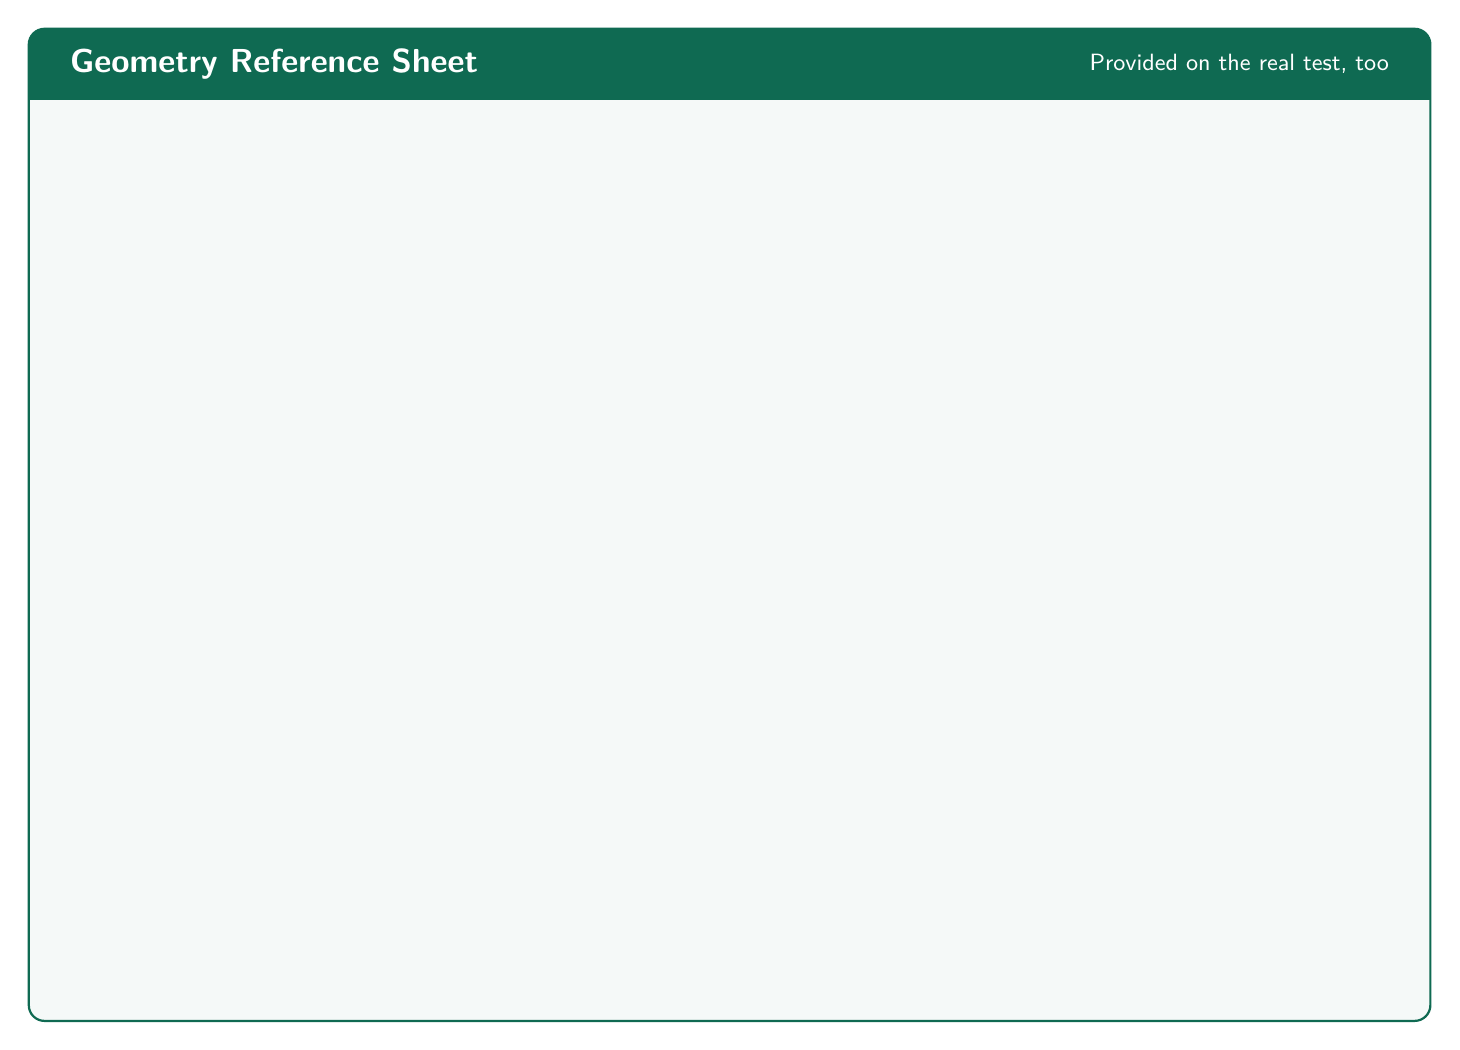
\begin{tikzpicture}
\draw[accent,line width=0.8pt,rounded corners=2mm,fill=badge!12] (0,0) rectangle (178mm,-126mm);
\fill[accent,rounded corners=2mm] (0,0) rectangle (178mm,-9mm);
\fill[accent] (0,-5mm) rectangle (178mm,-9mm);
\node[anchor=west,text=white,font=\sffamily\bfseries\fontsize{12}{14}\selectfont] at (4mm,-4.5mm) {Geometry Reference Sheet};
\node[anchor=east,text=white,font=\sffamily\fontsize{8.5}{10}\selectfont] at (174mm,-4.5mm) {Provided on the real test, too};
\end{tikzpicture}
\end{textblock*}

\newcommand{\refcell}[3]{\begin{textblock*}{42mm}(#1mm,#2mm)\begin{minipage}[t][36mm][t]{42mm}\centering #3\end{minipage}\end{textblock*}}
\newcommand{\refin}[2]{\parbox[b][26mm][b]{42mm}{\centering #1}\par\vspace{1.6mm}{\fontsize{9.6}{11.5}\selectfont #2}}
\tikzset{rf/.style={ink,line width=0.65pt},lb/.style={font=\fontsize{8.5}{9.5}\selectfont,inner sep=1.2pt}}

% ---------- row 1
\refcell{18}{167}{\refin{\begin{tikzpicture}[scale=1.25]
\draw[rf] (0,0) circle (9mm); \draw[rf] (0,0)--(9mm,0); \fill[ink] (0,0) circle (0.7pt);
\node[lb,above] at (4.5mm,0) {$r$};
\end{tikzpicture}}{Circle\\$A=\pi r^{2}$,\; $C=2\pi r$}}
\refcell{62}{167}{\refin{\begin{tikzpicture}[scale=1.25]
\draw[rf] (0,0) rectangle (22mm,12mm);
\node[lb,below] at (11mm,0) {$\ell$}; \node[lb,right] at (22mm,6mm) {$w$};
\end{tikzpicture}}{Rectangle\\$A=\ell w$}}
\refcell{106}{167}{\refin{\begin{tikzpicture}[scale=1.25]
\draw[rf] (0,0)--(22mm,0)--(7mm,13mm)--cycle;
\draw[rf,dashed] (7mm,0)--(7mm,13mm);
\draw[rf] (7mm,0)++(0,1.8mm)--++(1.8mm,0)--++(0,-1.8mm);
\node[lb,below] at (11mm,0) {$b$}; \node[lb,left] at (7mm,6.5mm) {$h$};
\end{tikzpicture}}{Triangle\\$A=\tfrac12 bh$}}
\refcell{150}{167}{\refin{\begin{tikzpicture}[scale=1.25]
\draw[rf] (0,0)--(18mm,0)--(0,12mm)--cycle;
\draw[rf] (0,1.8mm)--(1.8mm,1.8mm)--(1.8mm,0);
\node[lb,below] at (9mm,0) {$a$}; \node[lb,left] at (0,6mm) {$b$}; \node[lb,above right] at (9mm,6mm) {$c$};
\end{tikzpicture}}{Right triangle\\$c^{2}=a^{2}+b^{2}$}}

% ---------- row 2
\refcell{18}{204}{\refin{\begin{tikzpicture}[scale=1.25]
\draw[rf] (0,0)--(19.053mm,0)--(0,11mm)--cycle;
\draw[rf] (0,1.8mm)--(1.8mm,1.8mm)--(1.8mm,0);
\node[lb,below] at (9.5mm,0) {$x\sqrt3$}; \node[lb,left] at (0,5.5mm) {$x$}; \node[lb,above right] at (9.5mm,5.5mm) {$2x$};
\node[lb] at (14.6mm,1.9mm) {\fontsize{6.5}{7}\selectfont$30^\circ$}; \node[lb] at (3.2mm,8.2mm) {\fontsize{6.5}{7}\selectfont$60^\circ$};
\end{tikzpicture}}{$30^\circ$--$60^\circ$--$90^\circ$ triangle}}
\refcell{62}{204}{\refin{\begin{tikzpicture}[scale=1.25]
\draw[rf] (0,0)--(10mm,0)--(0,10mm)--cycle;
\draw[rf] (0,1.8mm)--(1.8mm,1.8mm)--(1.8mm,0);
\node[lb,below] at (5mm,0) {$s$}; \node[lb,left] at (0,5mm) {$s$}; \node[lb,above right] at (5mm,5mm) {$s\sqrt2$};
\end{tikzpicture}}{$45^\circ$--$45^\circ$--$90^\circ$ triangle}}
\refcell{106}{204}{\refin{\begin{tikzpicture}[scale=1.2]
\draw[rf] (0,0) rectangle (16mm,9mm);
\draw[rf] (16mm,9mm)--(22mm,13mm)--(6mm,13mm)--(0,9mm);
\draw[rf] (16mm,0)--(22mm,4mm)--(22mm,13mm);
\draw[rf,dashed] (6mm,13mm)--(6mm,4mm)--(22mm,4mm); \draw[rf,dashed] (0,0)--(6mm,4mm);
\node[lb,below] at (8mm,0) {$\ell$}; \node[lb,right] at (22mm,8.5mm) {$h$}; \node[lb,below right] at (19mm,2mm) {$w$};
\end{tikzpicture}}{Rectangular solid\\$V=\ell wh$}}
\refcell{150}{204}{\refin{\begin{tikzpicture}[scale=1.2]
\draw[rf] (0,2.2mm) ellipse (7mm and 2.2mm);
\draw[rf] (-7mm,2.2mm)--(-7mm,14mm); \draw[rf] (7mm,2.2mm)--(7mm,14mm);
\draw[rf] (0,14mm) ellipse (7mm and 2.2mm);
\draw[rf,dashed] (0,14mm)--(7mm,14mm); \fill[ink] (0,14mm) circle (0.6pt);
\node[lb,above] at (3.5mm,14mm) {$r$}; \node[lb,right] at (7mm,8mm) {$h$};
\end{tikzpicture}}{Right circular cylinder\\$V=\pi r^{2}h$}}

% ---------- row 3
\refcell{18}{241}{\refin{\begin{tikzpicture}[scale=1.15]
\draw[rf] (0,0) circle (10mm);
\draw[rf] (-10mm,0) arc (180:360:10mm and 2.8mm); \draw[rf,dashed] (-10mm,0) arc (180:0:10mm and 2.8mm);
\draw[rf] (0,0)--(10mm,0); \fill[ink] (0,0) circle (0.7pt); \node[lb,above] at (5mm,0) {$r$};
\end{tikzpicture}}{Sphere\\$V=\tfrac43\pi r^{3}$}}
\refcell{62}{241}{\refin{\begin{tikzpicture}[scale=1.2]
\draw[rf] (0,2.2mm) ellipse (7mm and 2.2mm);
\draw[rf] (-7mm,2.2mm)--(0,16mm)--(7mm,2.2mm);
\draw[rf,dashed] (0,16mm)--(0,2.2mm); \draw[rf,dashed] (0,2.2mm)--(7mm,2.2mm);
\fill[ink] (0,2.2mm) circle (0.6pt);
\node[lb,left] at (0,9.5mm) {$h$}; \node[lb,above] at (3.5mm,2.2mm) {$r$};
\end{tikzpicture}}{Right circular cone\\$V=\tfrac13\pi r^{2}h$}}
\refcell{106}{241}{\refin{\begin{tikzpicture}[scale=1.2]
\draw[rf] (0,0)--(16mm,0)--(22mm,4mm); \draw[rf] (0,0)--(10mm,15mm)--(16mm,0); \draw[rf] (10mm,15mm)--(22mm,4mm);
\draw[rf,dashed] (0,0)--(6mm,4mm)--(22mm,4mm); \draw[rf,dashed] (6mm,4mm)--(10mm,15mm);
\node[lb,below] at (8mm,0) {$\ell$}; \node[lb,below right] at (19mm,2mm) {$w$}; \node[lb,left] at (10mm,9.5mm) {$h$};
\end{tikzpicture}}{Rectangular pyramid\\$V=\tfrac13\ell wh$}}
\begin{textblock*}{40mm}(151mm,247mm)
{\fontsize{9.2}{12}\selectfont\raggedright
\textcolor{accent}{\rule[0.3mm]{1.6mm}{1.6mm}}\; A circle has 360 degrees of arc.\par\vspace{1.2mm}
\textcolor{accent}{\rule[0.3mm]{1.6mm}{1.6mm}}\; The angles of a triangle add up to 180 degrees.\par\vspace{1.2mm}
\textcolor{accent}{\rule[0.3mm]{1.6mm}{1.6mm}}\; $r$ radius, $\ell$ length, $w$ width, $b$ base, $h$ height.\par}
\end{textblock*}

\clearpage

% ===== Module 1, page 1 =====
\topicheader{3}{Mock Test 3}
\pagefooter{2}
\colrule{34}{236}
\mbox{}%
\pagekicker{Mock 3 \textperiodcentered{} Module 1 \textperiodcentered{} 22 questions \textperiodcentered{} 35 minutes}{Questions 1--8}
\begin{textblock*}{\COLW}(\LCOL,34mm)
{\fontsize{10.4}{13.4}\selectfont
\parbox[t][233mm][t]{\COLW}{%
\noindent\pnum{1} If $4x+9=33$, what is the value of $2x$?\par\vspace{2.2mm}
\hspace*{7mm}(A)\ $6$\\[1.8mm]
\hspace*{7mm}(B)\ $12$\\[1.8mm]
\hspace*{7mm}(C)\ $24$\\[1.8mm]
\hspace*{7mm}(D)\ $42$
\vfill

\noindent\pnum{2} Which expression is equivalent to $(5x^2-3x+2)-(2x^2-7x-1)$?\par\vspace{2.2mm}
\hspace*{7mm}(A)\ $3x^2-10x+1$\\[1.8mm]
\hspace*{7mm}(B)\ $7x^2+4x+3$\\[1.8mm]
\hspace*{7mm}(C)\ $3x^2+4x+1$\\[1.8mm]
\hspace*{7mm}(D)\ $3x^2+4x+3$
\vfill

\noindent\pnum{3} A vitamin syrup is 15\% sugar by volume. How many milliliters of sugar are in a 240-milliliter bottle of the syrup?\gridbox
\vfill

\noindent\pnum{4} A cylindrical can has a radius of 3 centimeters and a height of 10 centimeters. What is the volume of the can, in cubic centimeters?\par\vspace{2.2mm}
\hspace*{7mm}(A)\ $30\pi$\\[1.8mm]
\hspace*{7mm}(B)\ $60\pi$\\[1.8mm]
\hspace*{7mm}(C)\ $90\pi$\\[1.8mm]
\hspace*{7mm}(D)\ $360\pi$
\vfill}}
\end{textblock*}
\begin{textblock*}{\COLW}(\RCOL,34mm)
{\fontsize{10.4}{13.4}\selectfont
\parbox[t][233mm][t]{\COLW}{%
\noindent\pnum{5} In the $xy$-plane, the graph of $3x+4y=24$ crosses the $y$-axis at the point $(0,b)$. What is the value of $b$?\par\vspace{2.2mm}
\hspace*{7mm}(A)\ $6$\\[1.8mm]
\hspace*{7mm}(B)\ $8$\\[1.8mm]
\hspace*{7mm}(C)\ $12$\\[1.8mm]
\hspace*{7mm}(D)\ $24$
\vfill

\noindent\pnum{6} For $x>0$, which expression is equivalent to $\dfrac{(x^5)^2}{x^3}$?\par\vspace{2.2mm}
\hspace*{7mm}(A)\ $x^{10/3}$\\[1.8mm]
\hspace*{7mm}(B)\ $x^{4}$\\[1.8mm]
\hspace*{7mm}(C)\ $x^{7}$\\[1.8mm]
\hspace*{7mm}(D)\ $x^{13}$
\vfill

\noindent\pnum{7} If $5(x+2)=3x+20$, what is the value of $x$?\gridbox
\vfill

\noindent\pnum{8} The graph of a quadratic function in the $xy$-plane crosses the $x$-axis at $x=-4$ and $x=6$. What is the $x$-coordinate of the vertex of the graph?\par\vspace{2.2mm}
\hspace*{7mm}(A)\ $1$\\[1.8mm]
\hspace*{7mm}(B)\ $2$\\[1.8mm]
\hspace*{7mm}(C)\ $5$\\[1.8mm]
\hspace*{7mm}(D)\ $10$
\vfill}}
\end{textblock*}
\clearpage

% ===== Module 1, page 2 =====
\topicheader{3}{Mock Test 3}
\pagefooter{3}
\colrule{34}{236}
\mbox{}%
\pagekicker{Mock 3 \textperiodcentered{} Module 1 \textperiodcentered{} 22 questions \textperiodcentered{} 35 minutes}{Questions 9--16}
\begin{textblock*}{\COLW}(\LCOL,34mm)
{\fontsize{10.4}{13.4}\selectfont
\parbox[t][233mm][t]{\COLW}{%
\noindent\pnum{9} A small clinic's total monthly cost, in dollars, is modeled by $C(n)=4200+26n$, where $n$ is the number of patients the clinic sees in a month. Which of the following is the best interpretation of the number 26 in this context?\par\vspace{2.2mm}
\hspace*{7mm}(A)\ The clinic's fixed monthly cost is \$26.\\[1.8mm]
\hspace*{7mm}(B)\ The clinic sees 26 patients each month.\\[1.8mm]
\hspace*{7mm}(C)\ The clinic's monthly cost increases by \$4,200 for every 26 patients seen.\\[1.8mm]
\hspace*{7mm}(D)\ Each additional patient seen increases the clinic's monthly cost by \$26.
\vfill

\noindent\pnum{10} A patient is given 480 milligrams of a medication. The amount of the medication in the patient's body decreases by half every 5 hours. According to this model, how many milligrams of the medication remain after 15 hours?\par\vspace{2.2mm}
\hspace*{7mm}(A)\ $30$\\[1.8mm]
\hspace*{7mm}(B)\ $60$\\[1.8mm]
\hspace*{7mm}(C)\ $96$\\[1.8mm]
\hspace*{7mm}(D)\ $160$
\vfill

\noindent\pnum{11} A small business sells handmade candles for \$38 each. Its cost to make $n$ candles in a month is \$14 per candle plus a fixed monthly cost of \$4,800. What is the least number of candles the business must sell in a month for its revenue to be greater than its cost?\gridbox
\vfill

\noindent\pnum{12} A study of adults relates the number of minutes of exercise per week, $x$, to resting heart rate, $y$, in beats per minute. The line of best fit is $y=78-0.04x$. One adult in the study exercised 300 minutes per week and had a resting heart rate of 62 beats per minute. What is the residual for this adult (actual value minus predicted value), in beats per minute?\par\vspace{2.2mm}
\hspace*{7mm}(A)\ $-16$\\[1.8mm]
\hspace*{7mm}(B)\ $-12$\\[1.8mm]
\hspace*{7mm}(C)\ $-4$\\[1.8mm]
\hspace*{7mm}(D)\ $4$
\vfill}}
\end{textblock*}
\begin{textblock*}{\COLW}(\RCOL,34mm)
{\fontsize{10.4}{13.4}\selectfont
\parbox[t][233mm][t]{\COLW}{%
\noindent\pnum{13} The polynomial $p(x)=2x^3-5x^2+kx+6$ has $x+2$ as a factor, where $k$ is a constant. What is the value of $k$?\par\vspace{2.2mm}
\hspace*{7mm}(A)\ $-15$\\[1.8mm]
\hspace*{7mm}(B)\ $-1$\\[1.8mm]
\hspace*{7mm}(C)\ $2$\\[1.8mm]
\hspace*{7mm}(D)\ $15$
\vfill

\noindent\pnum{14} A sector of a circle has a central angle of $72^\circ$ and an area of $20\pi$ square units. What is the radius of the circle, in units?\gridbox
\vfill

\noindent\pnum{15} A hiker climbing at a constant rate was at an elevation of 1,350 meters after 2 hours and at an elevation of 1,830 meters after 5 hours. What was the hiker's elevation, in meters, after 9 hours?\par\vspace{2.2mm}
\hspace*{7mm}(A)\ $2{,}310$\\[1.8mm]
\hspace*{7mm}(B)\ $2{,}470$\\[1.8mm]
\hspace*{7mm}(C)\ $2{,}630$\\[1.8mm]
\hspace*{7mm}(D)\ $2{,}790$
\vfill

\noindent\pnum{16} If $4^{x}=8^{x-2}$, what is the value of $x$?\par\vspace{2.2mm}
\hspace*{7mm}(A)\ $-6$\\[1.8mm]
\hspace*{7mm}(B)\ $\dfrac{6}{5}$\\[1.8mm]
\hspace*{7mm}(C)\ $2$\\[1.8mm]
\hspace*{7mm}(D)\ $6$
\vfill}}
\end{textblock*}
\clearpage

% ===== Module 1, page 3 =====
\topicheader{3}{Mock Test 3}
\pagefooter{4}
\colrule{34}{236}
\mbox{}%
\pagekicker{Mock 3 \textperiodcentered{} Module 1 \textperiodcentered{} 22 questions \textperiodcentered{} 35 minutes}{Questions 17--22}
\begin{textblock*}{\COLW}(\LCOL,34mm)
{\fontsize{10.4}{13.4}\selectfont
\parbox[t][233mm][t]{\COLW}{%
\noindent\pnum{17} In the $xy$-plane, a line passes through the point $(0,-3)$ and is perpendicular to the graph of $y=2x+5$. Which equation represents the line?\par\vspace{2.2mm}
\hspace*{7mm}(A)\ $y=-\dfrac12x-3$\\[1.8mm]
\hspace*{7mm}(B)\ $y=\dfrac12x-3$\\[1.8mm]
\hspace*{7mm}(C)\ $y=-2x-3$\\[1.8mm]
\hspace*{7mm}(D)\ $y=2x-3$
\vfill

\noindent\pnum{18} A store's weekly revenue, in dollars, from selling a gadget at a price of $p$ dollars is modeled by $R(p)=500p-10p^2$ for $0<p<50$. What is the least price, in dollars, at which the weekly revenue is exactly \$4,000?\gridbox
\vfill

\noindent\pnum{19} The table shows the results for 300 patients at a clinic during one flu season. A patient who got the flu is selected at random. What is the probability that the patient had been vaccinated?\figwrap{\begin{tabular}{|l|c|c|}
\hline
 & Got the flu & Did not get the flu\\\hline
Vaccinated & 18 & 162\\\hline
Not vaccinated & 36 & 84\\\hline
\end{tabular}}\par\vspace{2.2mm}
\hspace*{7mm}(A)\ $\dfrac{3}{50}$\\[1.8mm]
\hspace*{7mm}(B)\ $\dfrac{1}{10}$\\[1.8mm]
\hspace*{7mm}(C)\ $\dfrac{3}{10}$\\[1.8mm]
\hspace*{7mm}(D)\ $\dfrac{1}{3}$
\vfill}}
\end{textblock*}
\begin{textblock*}{\COLW}(\RCOL,34mm)
{\fontsize{10.4}{13.4}\selectfont
\parbox[t][233mm][t]{\COLW}{%
\noindent\pnum{20} A car radiator holds 40 liters of coolant that is 25\% antifreeze. A mechanic drains some of the coolant and refills the radiator to 40 liters with pure antifreeze, so that the new mixture is 40\% antifreeze. How many liters of coolant did the mechanic drain?\par\vspace{2.2mm}
\hspace*{7mm}(A)\ $6$\\[1.8mm]
\hspace*{7mm}(B)\ $8$\\[1.8mm]
\hspace*{7mm}(C)\ $10$\\[1.8mm]
\hspace*{7mm}(D)\ $16$
\vfill

\noindent\pnum{21} A hemispherical bowl has an inside radius of 10 centimeters and sits with its rim facing up. Water in the bowl is 4 centimeters deep at the deepest point. What is the radius, in centimeters, of the circular surface of the water?\gridbox
\vfill

\noindent\pnum{22} What is the sum of the squares of all real solutions of the equation $2x^4-17x^2+8=0$?\par\vspace{2.2mm}
\hspace*{7mm}(A)\ $0$\\[1.8mm]
\hspace*{7mm}(B)\ $\dfrac{17}{2}$\\[1.8mm]
\hspace*{7mm}(C)\ $17$\\[1.8mm]
\hspace*{7mm}(D)\ $34$
\vfill}}
\end{textblock*}
\clearpage

% ===== Module 2, page 1 =====
\topicheader{3}{Mock Test 3}
\pagefooter{5}
\colrule{34}{236}
\mbox{}%
\pagekicker{Mock 3 \textperiodcentered{} Module 2 \textperiodcentered{} 22 questions \textperiodcentered{} 35 minutes}{Questions 1--8}
\begin{textblock*}{\COLW}(\LCOL,34mm)
{\fontsize{10.4}{13.4}\selectfont
\parbox[t][233mm][t]{\COLW}{%
\noindent\pnum{1} What is the solution to the equation $\dfrac{x+8}{3}=2x-4$?\par\vspace{2.2mm}
\hspace*{7mm}(A)\ $2$\\[1.8mm]
\hspace*{7mm}(B)\ $\dfrac{12}{5}$\\[1.8mm]
\hspace*{7mm}(C)\ $3$\\[1.8mm]
\hspace*{7mm}(D)\ $4$
\vfill

\noindent\pnum{2} Which expression is equivalent to $(3x-2)(x+5)$?\par\vspace{2.2mm}
\hspace*{7mm}(A)\ $3x^2+13x-10$\\[1.8mm]
\hspace*{7mm}(B)\ $3x^2+17x-10$\\[1.8mm]
\hspace*{7mm}(C)\ $3x^2+13x+10$\\[1.8mm]
\hspace*{7mm}(D)\ $3x^2-10$
\vfill

\noindent\pnum{3} Plan A for cell-phone service charges a \$18 monthly fee plus \$0.12 per minute of calls. Plan B charges a \$30 monthly fee plus \$0.08 per minute of calls. For how many minutes of calls in a month do the two plans cost the same amount?\gridbox
\vfill

\noindent\pnum{4} If $2^{x+3}+2^{x}=72$, what is the value of $x$?\par\vspace{2.2mm}
\hspace*{7mm}(A)\ $2$\\[1.8mm]
\hspace*{7mm}(B)\ $3$\\[1.8mm]
\hspace*{7mm}(C)\ $8$\\[1.8mm]
\hspace*{7mm}(D)\ $9$
\vfill}}
\end{textblock*}
\begin{textblock*}{\COLW}(\RCOL,34mm)
{\fontsize{10.4}{13.4}\selectfont
\parbox[t][233mm][t]{\COLW}{%
\noindent\pnum{5} The ratio of nurses to doctors on a hospital's staff is 7 to 2. After 12 nurses leave and 6 doctors join, the ratio of nurses to doctors is 5 to 3. How many nurses and doctors are on the staff after these changes?\par\vspace{2.2mm}
\hspace*{7mm}(A)\ $30$\\[1.8mm]
\hspace*{7mm}(B)\ $42$\\[1.8mm]
\hspace*{7mm}(C)\ $48$\\[1.8mm]
\hspace*{7mm}(D)\ $54$
\vfill

\noindent\pnum{6} In triangle $ABC$, $AB=AC=13$ and $BC=10$. What is the area of triangle $ABC$?\par\vspace{2.2mm}
\hspace*{7mm}(A)\ $60$\\[1.8mm]
\hspace*{7mm}(B)\ $65$\\[1.8mm]
\hspace*{7mm}(C)\ $120$\\[1.8mm]
\hspace*{7mm}(D)\ $130$
\vfill

\noindent\pnum{7} Ana cycles along a straight path at a constant 12 kilometers per hour. Thirty minutes after Ana leaves, Ben leaves the same starting point and rides along the same path at a constant 20 kilometers per hour. How many minutes after Ben leaves does he catch up to Ana?\par\vspace{2.2mm}
\hspace*{7mm}(A)\ $11.25$\\[1.8mm]
\hspace*{7mm}(B)\ $18$\\[1.8mm]
\hspace*{7mm}(C)\ $30$\\[1.8mm]
\hspace*{7mm}(D)\ $45$
\vfill

\noindent\pnum{8} The function $f(x)=x^2-8x+k$, where $k$ is a constant, has a minimum value of $-3$. What is the value of $k$?\par\vspace{2.2mm}
\hspace*{7mm}(A)\ $-3$\\[1.8mm]
\hspace*{7mm}(B)\ $3$\\[1.8mm]
\hspace*{7mm}(C)\ $13$\\[1.8mm]
\hspace*{7mm}(D)\ $19$
\vfill}}
\end{textblock*}
\clearpage

% ===== Module 2, page 2 =====
\topicheader{3}{Mock Test 3}
\pagefooter{6}
\colrule{34}{236}
\mbox{}%
\pagekicker{Mock 3 \textperiodcentered{} Module 2 \textperiodcentered{} 22 questions \textperiodcentered{} 35 minutes}{Questions 9--16}
\begin{textblock*}{\COLW}(\LCOL,34mm)
{\fontsize{10.4}{13.4}\selectfont
\parbox[t][233mm][t]{\COLW}{%
\noindent\pnum{9} The number of cells in a laboratory culture $t$ hours after the start of an experiment is modeled by $N(t)=250\cdot3^{t/4}$. According to the model, at what value of $t$ will there be 6,750 cells in the culture?\gridbox
\vfill

\noindent\pnum{10} Which ordered pair $(x,y)$ is a solution to the system of inequalities below?\dsp{$y>2x-3$}\dsp{$y\le -x+6$}\par\vspace{2.2mm}
\hspace*{7mm}(A)\ $(1,6)$\\[1.8mm]
\hspace*{7mm}(B)\ $(3,3)$\\[1.8mm]
\hspace*{7mm}(C)\ $(4,2)$\\[1.8mm]
\hspace*{7mm}(D)\ $(2,3)$
\vfill

\noindent\pnum{11} What is the sum of all real solutions of the equation below?\dsp{$\dfrac{x^2}{x-6}=\dfrac{36}{x-6}$}\par\vspace{2.2mm}
\hspace*{7mm}(A)\ $-6$\\[1.8mm]
\hspace*{7mm}(B)\ $0$\\[1.8mm]
\hspace*{7mm}(C)\ $6$\\[1.8mm]
\hspace*{7mm}(D)\ $12$
\vfill

\noindent\pnum{12} In the equation $(a-2)x+14=5x+2a$, $a$ is a constant. If the equation has infinitely many solutions, what is the value of $a$?\gridbox
\vfill}}
\end{textblock*}
\begin{textblock*}{\COLW}(\RCOL,34mm)
{\fontsize{10.4}{13.4}\selectfont
\parbox[t][233mm][t]{\COLW}{%
\noindent\pnum{13} In a clinical trial, 600 volunteers were assigned to either a drug group of 360 volunteers or a placebo group of the remaining volunteers. In the drug group, the number of volunteers whose symptoms improved was 3 times the number whose symptoms did not improve. Overall, 330 of the 600 volunteers improved. If one volunteer whose symptoms did not improve is selected at random, what is the probability that the volunteer was in the placebo group?\par\vspace{2.2mm}
\hspace*{7mm}(A)\ $\dfrac{3}{10}$\\[1.8mm]
\hspace*{7mm}(B)\ $\dfrac{1}{3}$\\[1.8mm]
\hspace*{7mm}(C)\ $\dfrac{2}{3}$\\[1.8mm]
\hspace*{7mm}(D)\ $\dfrac{3}{4}$
\vfill

\noindent\pnum{14} A bakery's daily production cost, in dollars, is a linear function of the number of loaves baked. When 400 loaves are baked in a day, the average cost per loaf is \$19.00. When 500 loaves are baked in a day, the average cost per loaf is \$17.60. What is the bakery's fixed daily cost, in dollars?\par\vspace{2.2mm}
\hspace*{7mm}(A)\ $1{,}200$\\[1.8mm]
\hspace*{7mm}(B)\ $2{,}800$\\[1.8mm]
\hspace*{7mm}(C)\ $4{,}800$\\[1.8mm]
\hspace*{7mm}(D)\ $7{,}600$
\vfill

\noindent\pnum{15} A biologist models the height of a seedling with the line of best fit $H=3.2+0.85d$, where $H$ is the height in centimeters and $d$ is the number of days after planting. A second researcher begins measuring 14 days after planting and records the same seedling's height, $M$, in millimeters, as a function of $w$, the number of weeks since the second researcher began measuring. Which equation expresses the same line of best fit in terms of $M$ and $w$?\par\vspace{2.2mm}
\hspace*{7mm}(A)\ $M=15.1+5.95w$\\[1.8mm]
\hspace*{7mm}(B)\ $M=32+59.5w$\\[1.8mm]
\hspace*{7mm}(C)\ $M=151+8.5w$\\[1.8mm]
\hspace*{7mm}(D)\ $M=151+59.5w$
\vfill

\noindent\pnum{16} A company sells $x$ units per day at a price of $p=120-2x$ dollars per unit. Producing the units costs \$20 per unit plus a fixed daily cost of $F$ dollars. For one particular value of $F$, there is exactly one production level $x$ at which the company's revenue equals its cost. What is that value of $F$?\par\vspace{2.2mm}
\hspace*{7mm}(A)\ $1{,}250$\\[1.8mm]
\hspace*{7mm}(B)\ $1{,}800$\\[1.8mm]
\hspace*{7mm}(C)\ $2{,}500$\\[1.8mm]
\hspace*{7mm}(D)\ $3{,}600$
\vfill}}
\end{textblock*}
\clearpage

% ===== Module 2, page 3 =====
\topicheader{3}{Mock Test 3}
\pagefooter{7}
\colrule{34}{236}
\mbox{}%
\pagekicker{Mock 3 \textperiodcentered{} Module 2 \textperiodcentered{} 22 questions \textperiodcentered{} 35 minutes}{Questions 17--22}
\begin{textblock*}{\COLW}(\LCOL,34mm)
{\fontsize{10.4}{13.4}\selectfont
\parbox[t][233mm][t]{\COLW}{%
\noindent\pnum{17} A cube with an edge length of 6 centimeters is placed inside a sphere so that all 8 vertices of the cube lie on the sphere. What is the volume of the sphere, in cubic centimeters?\par\vspace{2.2mm}
\hspace*{7mm}(A)\ $36\pi$\\[1.8mm]
\hspace*{7mm}(B)\ $72\sqrt2\,\pi$\\[1.8mm]
\hspace*{7mm}(C)\ $108\sqrt3\,\pi$\\[1.8mm]
\hspace*{7mm}(D)\ $288\pi$
\vfill

\noindent\pnum{18} In the $xy$-plane, line $\ell$ passes through the point $(2,5)$, and line $n$ passes through the point $(8,-3)$. Lines $\ell$ and $n$ are perpendicular and intersect at a point on the $y$-axis. What is the slope of $\ell$?\par\vspace{2.2mm}
\hspace*{7mm}(A)\ $-\dfrac12$\\[1.8mm]
\hspace*{7mm}(B)\ $2$\\[1.8mm]
\hspace*{7mm}(C)\ $4$\\[1.8mm]
\hspace*{7mm}(D)\ $8$
\vfill

\noindent\pnum{19} The graph of the quadratic function $f$ in the $xy$-plane has its vertex at $(4,-12)$ and passes through the point $(0,20)$. The function $g$ is defined by $g(x)=f\!\left(\frac{x}{2}\right)$. What is the distance between the two $x$-intercepts of the graph of $g$?\par\vspace{2.2mm}
\hspace*{7mm}(A)\ $\sqrt6$\\[1.8mm]
\hspace*{7mm}(B)\ $2\sqrt6$\\[1.8mm]
\hspace*{7mm}(C)\ $8$\\[1.8mm]
\hspace*{7mm}(D)\ $4\sqrt6$
\vfill}}
\end{textblock*}
\begin{textblock*}{\COLW}(\RCOL,34mm)
{\fontsize{10.4}{13.4}\selectfont
\parbox[t][233mm][t]{\COLW}{%
\noindent\pnum{20} For each integer value of $k$, the lines $kx+3y=12$ and $2x-y=5$ are graphed in the $xy$-plane. For how many integer values of $k$ do the two lines intersect at a point in the first quadrant (where both coordinates are positive)?\gridbox
\vfill

\noindent\pnum{21} A circle is inscribed in a right triangle so that it is tangent to all three sides of the triangle. The hypotenuse of the triangle is 26 units long, and the perimeter of the triangle is 60 units. What is the radius, in units, of the circle?\par\vspace{2.2mm}
\hspace*{7mm}(A)\ $2$\\[1.8mm]
\hspace*{7mm}(B)\ $4$\\[1.8mm]
\hspace*{7mm}(C)\ $8$\\[1.8mm]
\hspace*{7mm}(D)\ $13$
\vfill

\noindent\pnum{22} If $4^{x}+4^{-x}=7$, what is the value of $2^{x}+2^{-x}$?\gridbox
\vfill}}
\end{textblock*}
\clearpage

\end{document}
